\documentclass[12pt,a4paper]{article}
\usepackage{ctex}
\usepackage{amsmath,amscd,amsbsy,amssymb,latexsym,url,bm,amsthm}
\usepackage{epsfig,graphicx,subfigure}
\usepackage{enumitem,balance}
\usepackage{wrapfig}
\usepackage{mathrsfs,euscript}
\usepackage[usenames]{xcolor}
\usepackage{hyperref}
\usepackage[vlined,ruled,linesnumbered]{algorithm2e}
\usepackage{float}
\hypersetup{colorlinks=true,linkcolor=black}

\newtheorem{theorem}{Theorem}
\newtheorem{lemma}[theorem]{Lemma}
\newtheorem{proposition}[theorem]{Proposition}
\newtheorem{corollary}[theorem]{Corollary}
\newtheorem{exercise}{Exercise}
\newtheorem*{solution}{Solution}
\newtheorem{definition}{Definition}
\theoremstyle{definition}

\renewcommand{\thefootnote}{\fnsymbol{footnote}}

\newcommand{\postscript}[2]
 {\setlength{\epsfxsize}{#2\hsize}
  \centerline{\epsfbox{#1}}}

\renewcommand{\baselinestretch}{1.0}

\setlength{\oddsidemargin}{-0.365in}
\setlength{\evensidemargin}{-0.365in}
\setlength{\topmargin}{-0.3in}
\setlength{\headheight}{0in}
\setlength{\headsep}{0in}
\setlength{\textheight}{10.1in}
\setlength{\textwidth}{7in}
\makeatletter \renewenvironment{proof}[1][Proof] {\par\pushQED{\qed}\normalfont\topsep6\p@\@plus6\p@\relax\trivlist\item[\hskip\labelsep\bfseries#1\@addpunct{.}]\ignorespaces}{\popQED\endtrivlist\@endpefalse} \makeatother
\makeatletter
\renewenvironment{solution}[1][Solution] {\par\pushQED{\qed}\normalfont\topsep6\p@\@plus6\p@\relax\trivlist\item[\hskip\labelsep\bfseries#1\@addpunct{.}]\ignorespaces}{\popQED\endtrivlist\@endpefalse} \makeatother

\begin{document}
\noindent

%========================================================================
\noindent\framebox[\linewidth]{\shortstack[c]{
\Large{\textbf{Lab03-GreedyStrategy}}\vspace{1mm}\\
CS214-Algorithm and Complexity, Xiaofeng Gao, Spring 2020.}}
\begin{center}
\footnotesize{\color{red}$*$ If there is any problem, please contact TA Shuodian Yu.}

% Please write down your name, student id and email.
\footnotesize{\color{blue}$*$ Name:Hanzhang Yang  \quad Student ID:518030910022 \quad Email: linqinluli@sjtu.edu.cn}
\end{center}

\begin{enumerate}
    \item
    There are $n+1$ people, each with two attributes $(a_i,b_i), i\in[0,n] \text{ and } a_i>1$. The $i$-th person can get money worth $c_i = \frac{\prod_{j=0}^{i-1}{a_j}}{b_i}$. We do not want anyone to get too much. Thus, please design a strategy to sort people from $1$ to $n$, such that the maximum earned money $c_{max}=\max\limits_{1\leq i\leq n} c_i$ is minimized. (Note: the 0-th person doesn't enroll in the sorting process, but $a_0$ always works for each $c_i$.)
    \begin{enumerate}
        \item Please design an algorithm based on greedy strategy to solve the above problem. (Write a pseudocode)
        \item Prove your algorithm is optimal.
    \end{enumerate}

    (a).

    \begin{algorithm}[H]
        \KwIn{Array $A[a_0,a_1,\cdots,a_{n}]$, array $B[b_0,b_2,\cdots,b_{n}]$}
        \KwOut{sorted array that makes max $c_i = \frac{\prod_{j=0}^{i-1}{a_j}}{b_i}$ minimized}
        \BlankLine
        $M=[1,2,\cdots,n]$\;
        Sort $M$ by $A[M[i]]\times B[M[i]]$ so that $A[M[1]]\times B[M[1]] \le A[M[2]]\times B[M[2]] \le \cdots \le A[M[n]]\times B[M[n]]$\;
        \textbf{Output} $M$\;
    \end{algorithm}
        
   (b).

    \begin{solution}
        Consider two people next to each other. $(a_i,b_i),\ (a_{i+1},b_{i+1})$.

        Assume it's best when $a_i$ is before $a_{i+1}$. We can find that exchanging $a_i$ and $a_{i+1}$ won't affect other people.

        $S=\prod_{j=0}^{i-1} a_j$

        case 1 : $a_i$ is before $a_{i+1}$

        $c_i=\frac{S}{b_i}$

        $c_{i+1}=\frac{S\times a_i}{b_{i+1}}$

        case 2 : $a_{i+1}$ is before $a_{i}$

        $c_{i+1}=\frac{S}{b_{i+1}}$

        $c_i=\frac{S\times a_{i+1}}{b_{i}}$

        we can get $$max\{ \frac{S}{b_i},\frac{S\times a_i}{b_{i+1}} \} \le max \{ \frac{S}{b_{i+1}},\frac{S\times a_{i+1}}{b_{i}} \} $$

        $\frac{S}{b_i} \le \frac{S\times a_{i+1}}{b_{i}} , \ \frac{S\times a_i}{b_{i+1}} \ge \frac{S}{b_{i+1}}$
    
        Thus $\frac{S\times a_i}{b_{i+1}} \le \frac{S\times a_{i+1}}{b_{i}}\quad \rightarrow a_ib_i\le a_{i+1}b_{i+1}$
    
        Therefore it's best for all people to sort by $a_i\times b_i$
     \end{solution}

    \item
    \textbf{Interval Scheduling} is a classic problem solved by greedy algorithm and we have introduced it in the lecture: given $n$ jobs and the $j$-th job starts at $s_j$ and finishes at $f_j$. Two jobs are compatible if they do not overlap. The goal is to find maximum subset of mutually compatible jobs. Tim wants to solve it by sort the jobs in descending order of $s_j$. Is this attempt correct? Prove the correctness of such idea, or else provide a counter-example.

    Yes.

    \begin{proof}
        (By contradiction)
       Assume greedy is not optimal.

       Let $i_{n},i_{n-1},\cdots,i_{k}$ denote set of jobs selected by greedy.

       Let $j_n,j_{n-1},\cdots,j_{m}$ denote set of jobs in an optimal solution with $i_j=j_n,\cdots, i_r=j_r$ for the largest possible value of r.

       The $i_{r-1}$ is selected by Greedy, so job $i_{r-1}$ begins after $j_{r-1}$. 

       Thus we change $j_{r-1}$ to $i_{r-1}$. The solution of OPT is still feasible and optimal, but contradicts the maximality of r.
   
       \begin{figure}[H] 
        \centering 
        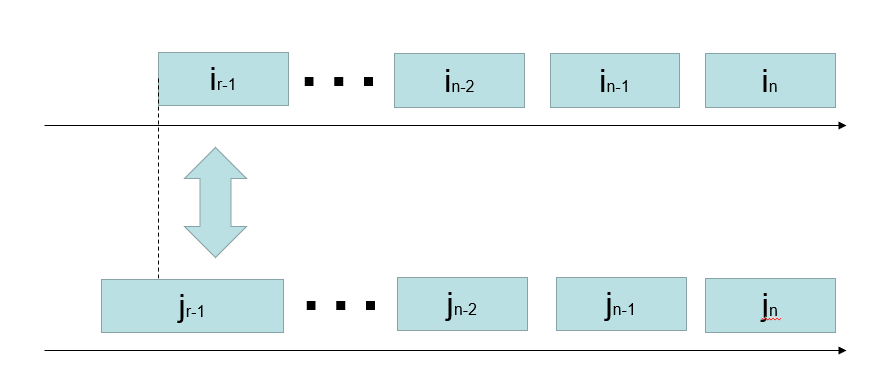
\includegraphics[width=0.7\textwidth]{greedy} 
        \label{wolf} 
    \end{figure}
       Therefore we can conclude that greedy is optimal.
    \end{proof}

    \item
    There are $n$ lectures numbered from $1$ to $n$. Lecture $i$ has duration (course length) $t_i$ and will close on $d_i$-th day. That is, you could take lecture $i$ \textbf{continuously} for $t_i$ days and must finish before or on the $d_i$-th day. The goal is to find the maximal number of courses that can be taken. (Note: you will start learning at the $1$-st day.)
    
    Please design an algorithm based on greedy strategy to solve it. You could use the data structrue learned on Data Structrue course. You need to write pseudo code and prove its correctness.

    \begin{algorithm}
        \KwIn{$A[(t_1,d_1),(t_2,d_2),\cdots,(t_n,d_n)]$}
        \KwOut{maximal number of courses that can be taken}
        \BlankLine
        sort $A$ that $d_1\le d_2 \le \cdots \le d_n$\\
        creat a max-heap M\\
        $M.push(A[1])$;\\
        $time=t_1$;\\
        $num=1;$\\
        \For{$i=2$ to $n$}{
            \uIf{$time+t_i>d_i$}{
                \uIf{$M.top().t>t_i$}{
                    $time=time-M.top().t+t_i;$\\
                    $M.pop();$\\
                    $M.push(A[i]);$\\
                    num++;\\
                }
                \Else{
                    continue;
                }
            }
            \Else{
                $num++;$\\
                $time=time+t_i$\\
                $M.push(A[i]);$\\
            }
        }
        \textbf{output} $num$\;

    \end{algorithm}
    
    \begin{solution}
        By induction.

        \textbf{Basis step.} When $n=1$, greedy=opt.

        \textbf{Induction Hypothesis.} Assume when $n=k$ greedy is opt.

        \textbf{Proof of Induction Step.} For the $k+1$ lecture, if $time+t_i\le d_i$. Greedy increases 1 the same as opt;
        When $time+t_i> d_i$, greedy choose smaller one between the lecture owning the largest time of all selected lectures and the $k+1_{th}$
        lecture. (Assume the largest one is on the $m_{th}$.) If exchange happened, since $d_{k+1}\le d_{m}$ and $t_{k+1}< t_m$, number of lectures
        won't change and the $time$ is smaller than before. Thus no matter whether the exchange would happen, the number and the time is sitll the best case.

        Therefore greedy is opt.
   \end{solution}

    \item
    Let $S_1,S_2,\dots,S_n$ be a partition of $S$ and $k_1,k_2,\dots,k_n$ be positive integers. Let $\mathcal{I}=\{I: I \subseteq S,|I \cap S_i| \leq k_i \text { for all } 1 \leq i \leq n\}$. Prove that $\mathcal{M}=(S,\mathcal{I})$ is a matroid.

    \begin{proof}
        
        \textbf{Hereditary:}

        Assume $A\subset B, B\in \mathcal{I}$.

        Since $A\subset B$,$B \subseteq S,|B \cap S_i| \leq k_i \text { for all } 1 \leq i \leq n\ $, $ A \subseteq S,|A \cap S_i| \leq k_i \text { for all } 1 \leq i \leq n\ $

        Thus $A\in \mathcal{I}$

        \textbf{Exchange Property:}

        Assume $A,B\in \mathcal{I}$, $|A|<|B|$ and $x\in B\backslash A$.

        For $A\subseteq S,\ B\subseteq S$, $A\cup \{ x \} \subseteq S.$
        
        \textbf{case 1:} $B\subseteq S_i$, $k_i\ge |B|$

        Thus $|A\cup \{ x\} |=|A|+1\le |B|\le k_i$, $A\cup \{ x\}\in \mathcal{I}$.

        \textbf{case 2:} $B \nsubseteq S_i$

        Make $x\in B\backslash S_i$. Thus $|A\cup \{ x\} |=|A|\le k_i$, $A\cup \{ x\}\in \mathcal{I}$.

        $\mathcal{M}=(S,\mathcal{I})$ is a matroid.

    \end{proof}

\end{enumerate}

\vspace{20pt}

\textbf{Remark:} You need to include your .pdf and .tex files in your uploaded .rar or .zip file.

%========================================================================
\end{document}
